\documentclass[12pt]{article}
\usepackage{cmbright}
\usepackage[margin=1in]{geometry}
\usepackage{fancyvrb}
\usepackage{amsmath}
\usepackage{graphics}

\newcommand{\keff}{k_{\text{eff}}}

\title{A trivial Monte Carlo eigenvalue calculation}
\author{James Paul Holloway}

\begin{document}

\maketitle

\section{Introduction}

Often, in order to understand a technique, we should reduce it to its simplest possible application, for if we can't understand it there, we can't understand it anywhere.  These notes outline the Monte Carlo approach to $k$-eigenvalue calculations in the simplest possible case: an infinite homogeneous medium.  Of course, the value of $\keff$ for such a system is known.  Using $\Sigma$ to denote macroscopic cross sections, and subscripts $f$ and $\gamma$ to denote fission and radiative capture, we have
\begin{equation}
\keff = k_\infty = \frac{\nu \Sigma_f}{\Sigma_a}
\end{equation}
where $\Sigma_a = \Sigma_f + \Sigma_\gamma$.


The ``transport equation'', such as it is in our simple case, is
\begin{equation}
\Sigma_t  \phi = {\nu \Sigma_f} \phi + \Sigma_s \phi \,,
\end{equation}
where $\Sigma_s$ is the scattering cross section and $\Sigma_t = \Sigma_a + \Sigma_s$.  The $k$ eigenvalue problem arises by scaling $\nu$ in such a way that this homogeneous equation supports a non-zero solution, so we consider
\begin{equation}
\Sigma_t  \phi = \frac{\nu \Sigma_f}{k} \phi + \Sigma_s \phi \,.
\end{equation}
Note that in this infinite homogeneous medium, the various ``operators'' of transport theory are just multiplication by various constants.

\section{Inverse power iteration}

Inverse power iteration for $k$ comes from isolating the $1/k$ scaled fission source
\begin{equation}
\Sigma_a  \phi = \frac{\nu \Sigma_f}{k} \phi \,.
\end{equation}
and ``inverting'' the transport operator on the left
\begin{equation}
\phi = \frac{1}{\Sigma_a} \biggl[\frac{\nu \Sigma_f}{k} \phi \biggr] = \frac{1}{k} \frac{1}{\Sigma_a} \biggl[Q \biggr]\,.  \label{eq:inverse}
\end{equation}
Note that if the fission source $Q = \nu\Sigma_f \phi$ is known, then evaluating the expression on the right simply requires solving a fixed source transport problem, a task to which Monte Carlo is well suited.

We can apply the fission operator (multiply by $\nu \Sigma_f$) to Eq.~\ref{eq:inverse} and arrive at
\begin{equation}
Q = \frac{1}{k} \frac{\nu\Sigma_f}{\Sigma_a} \biggl[Q \biggr] \label{eq:fp}
\end{equation}
This is identical to Martin's Eq. 2 in his 6/23/06 document, where his $M$ corresponds to my multiplication by $\nu\Sigma_f$, and his $A^{-1}$ to my division by $\Sigma_a$.  A Monte Carlo algorithm can evaluate $A^{-1}$, because that just means ``solve a fixed source problem,'' and it can tally the fission source that results from that solution in order to compute $MA^{-1}Q$. A Monte Carlo algorithm can also divide by $\Sigma_a$, as we will see, and such an algorithm can tally the effect of the multiplication by $\nu\Sigma_f$.

The inverse power iteration is then based on the iteration
\begin{equation}
Q^{n+1} = \frac{1}{k^n} \frac{\nu\Sigma_f}{\Sigma_a} \biggl[Q^n \biggr] \,.
\label{eq:Qiteration}
\end{equation}
To compute an update for $k$. in general we would take the inner product of Eq.~\ref{eq:fp} with some function $U$, converting it into a scalar equality, and solve for $k$.  Because we have only scalar operators it does not matter what ``$U$'' would be in this case, and we simply rearrange Eq.~\ref{eq:fp} into the form
\begin{equation}
k = \frac{\nu\Sigma_f \Sigma_a^{-1} Q}{Q} \,.
\end{equation} 
Then, we can compute
\begin{equation}
k^{n+1} = \frac{\nu\Sigma_f \Sigma_a^{-1} Q^n}{Q^n} \,.
\end{equation}
This can be simplified because, by Eq.~\ref{eq:Qiteration}, $\nu\Sigma_f \Sigma_a^{-1} Q^n = k^n Q^{n+1}$, and so 
\begin{equation}
k^{n+1} = k^n \frac{Q^{n+1}}{Q^n} \,.
\end{equation}
The complete iteration is thus
\begin{align}
Q^{n+1} &= \frac{1}{k^n} \frac{\nu\Sigma_f}{\Sigma_a} \biggl[Q^n \biggr] \label{eq:Qiter}\\
k^{n+1} &= k^n \frac{Q^{n+1}}{Q^n} \label{eq:kiter} \,.
\end{align}

\subsection{Convergence of the iteration}

It is easy to see that if $k_n = k_\infty$ then $Q^{n+1} = Q^n$ in Eq.~\ref{eq:Qiter} and then that $k^{n+1} = k^n = k_\infty$ in Eq.~\ref{eq:kiter}.  Thus, if the iteration converges, it converges to the correct result for $k$, and $Q$ is of course arbitrary.

Indeed, for any $Q_0, k_0$ we have
\begin{align}
Q^{1} &= \frac{1}{k^0} \frac{\nu\Sigma_f}{\Sigma_a} Q^0 = \frac{k_\infty}{k^0} Q^0\\
k^{1} &= k^0 \frac{Q^{1}}{Q^0} = k^0 \frac{k_\infty}{k^0} \frac{Q^0}{Q^0} = k_\infty \,.
\end{align}
In other words, the iteration will converge in one step! But what would a Monte Carlo implementation look like?

\subsection{Monte Carlo implementation}

At the start of each iteration we have an estimate for $Q^n$ and $k^n$.  In this infinite dimensional context $Q^n$ is just the number of fission neutrons that were released during iteration $n$.  To evaluate $Q^{n+1}$ we must compute the number of fission neutrons that are caused to be released by the known source $Q^n/k_n$.  But we must interpret this statement carefully; Eq.~\ref{eq:Qiter} says to take neutrons from the source $Q^n/k^n$, follow them until they are absorbed, and then to compute the fission source that would result from the implied flux.   The neutrons from \emph{this} source are \emph{not} transported as part of Eq.~\ref{eq:Qiter}.  We can equivalently say that we transport particles from the source $Q_n$, and when they are absorbed we compute the fission neutrons that they would release \emph{using a mean number of secondaries $\nu^n = \nu/k^n$}; we will use this latter view.

To solve Eq.~\ref{eq:Qiter} we select a number $N$ of histories to run per iteration (particles per cycle they say in the code world).  In our problem, all of our neutrons will be absorbed eventually (they have nowhere else to go).  When they are absorbed, the number, $m^n$, of fission neutrons released on average is $\nu/k^n$ times the probability of fission given that an absorption has occurred, or $m^n = (\nu/k^n) (\Sigma_f/\Sigma_a)$.  For reasons that have to do with the needs of space dependent cases, we need a pdf to sample that has this mean.  The one used is $p(s|m^n)$, where
\begin{equation}
p(s|m) = \begin{cases}
1 - (m - \lfloor m \rfloor) &s = \lfloor m \rfloor\\
(m - \lfloor m \rfloor) &s = \lfloor m \rfloor + 1\\
0&\text{otherwise}
\end{cases}
\end{equation}
where $s$ is the integer number of particles to be released in fission, and $\lfloor m \rfloor$ is the nearest integer less than or equal to $m$ (the floor function applied to $m$).  A direct calculation will show that $\langle s \rangle = m$ as desired.
To sample $p(s|m)$ for $s$, the expression
\begin{equation}
s = \bigl\lfloor m + \xi \bigr\rfloor
\end{equation}
is used, where $0 \leq \xi < 1$ is a uniformly distributed random number.

Note that the mean number of particles released per fission, $m^n$, and the pdf used to sample it, change from one iteration to the next because the mean number of secondaries $\nu^n = \nu/k_n$ varies from one iteration to the next.

\subsection{The Monte Carlo algorithm}

For each iteration (cycle) we:
\begin{enumerate}
\item Initialize a count of fission neutrons $\tilde Q^{n+1}$ to zero
\item compute 
\begin{equation}
m^n = \frac{\nu \Sigma_f}{\Sigma_a k^n}
\end{equation}
\item Then for each history in the iteration we 
sample $p(s|m^n)$, and add this sample $\tilde Q^{n+1}$.  
\item At the end of the $N$ histories, we can compute the tally
\begin{equation}
Q^{n+1} = \frac{\tilde Q^{n+1}}{N} Q^n \,.
\end{equation}
Note in this that we compute the number of fission neutrons released per source particle (divide by the number of histories), times the magnitude of the previous source.  
\item Finally, we can compute the new $k$ estimate
\begin{equation}
k^{n+1} = k^n \frac{Q^n \tilde Q^{n+1}/N}{Q^{n}} = k^n \frac{\tilde Q^{n+1}}{N} = k^n \frac{\text{number of fission neutrons banked}}{\text{particles per cycle}}
\end{equation}

\end{enumerate}

Note that the final two steps implement Eq.~\ref{eq:kiter}. We don't need Eq.~\ref{eq:Qiter} in this infinite medium case.

The algorithm can be compressed into, for each cycle,
\begin{enumerate}
\item Initialize a count of fission neutrons $\tilde Q^{n+1}$ to zero
\item For each history $\tilde Q^{n+1} = \tilde Q^{n+1} + \bigl\lfloor \nu \Sigma_f/({\Sigma_a k^n}) + \xi \bigr\rfloor$ 
\item At the end of the $N$ histories, we can compute the new $k$ estimate
\begin{equation}
k^{n+1} = k^n \frac{\tilde Q^{n+1}}{N} = k^n \frac{\text{number of fission neutrons banked}}{\text{particles per cycle}}
\end{equation}

\end{enumerate}


\section{The $k_\infty$ code}

The Matlab code below will implement the $k$ calculation.  It contains two methods, method 2 is what is described above.  Method 1 only contributes particles to the ``fission bank'' when there is a fission.  Because fewer particles contribute, it has a higher variance.  Here is a sample run:
\begin{Verbatim}
>> sigF = 1; sigG = 1; sigS = 0; nu = 2.5;
>> histPerCycle = 1000; cycles = 100;
>> k1 = kInfinity(histPerCycle, cycles, sigS, sigG, sigF, nu, 1);
>> k2 = kInfinity(histPerCycle, cycles, sigS, sigG, sigF, nu, 2);
>> 
\end{Verbatim}

Figure~\ref{fig:k1000} shows the $k$ estimates over the first 100 cycles, using 1000 histories per cycle.  Note that the results are as good as they are going to be in about one cycle, because the deterministic iteration needs only one iteration in this trivial case.  After that. it's just fluctuations.

\begin{figure}
\begin{center}
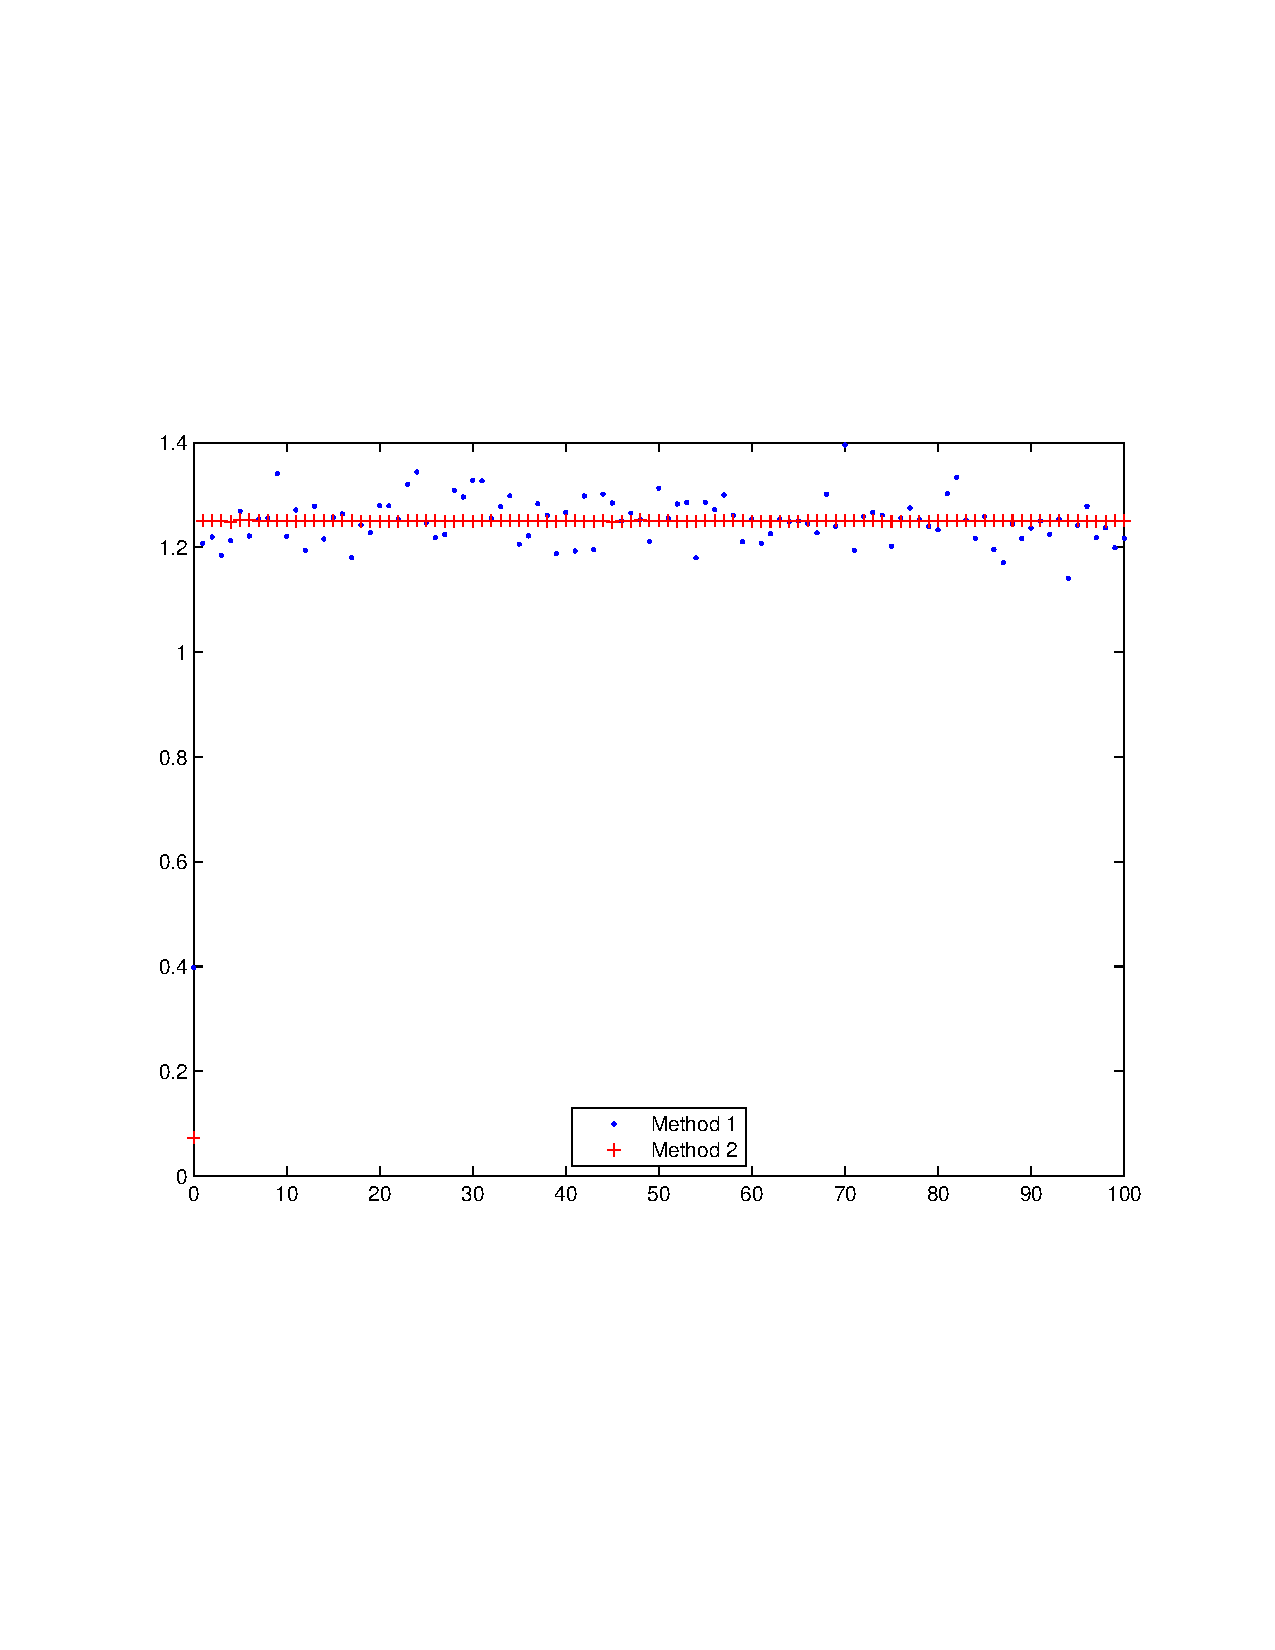
\includegraphics{k1000.pdf}
\end{center}
\caption{$k$ estimates computed using two methods, showing 100 cycles and using 1000 histories per cycle. The exact value is $k_\infty = 2.5 \times 1 / (1 + 1) = 1.25$.  Note that Method 2 is lower variance.  The spread in Method 1 will reduce with more particles per history.}
\label{fig:k1000}
\end{figure}

Here is the code to calculate $k_\infty$ by Monte Carlo.

{\small
\VerbatimInput{kinfinity.m}
}

\end{document}